\part{Polymorphism}
\frame{\partpage}

\begin{frame}{Introduction to Polymorphism}
	\begin{itemize}
		\pause \item Polymorphism is another key feature of OOP languages
		\pause \item The basic idea is that instances of a derived class can be treated as objects of the basic class
		\pause \item They can be used as parameters for functions and in collections
		\pause \item We then call the functions on these objects and our code will called the 'correct' version of the function
		\pause \item This is best illustrated by an example 
	\end{itemize}
\end{frame}


\begin{frame}[fragile]{Polymorphism example}
	\begin{lstlisting}[language=C++,basicstyle=\tiny,]
	class Enemy{/*This has been defined in previous slides*/}
	class Boss : Enemy{/*Again see previou slides*/}
	
	//This Function is called by any enemy to carry out an attack
	void DoAttacks(Enemy *enemy)
	{
		enemy->Attack();
	}
	
	//We probably have grabbed these from other game objects
	Enemy goblin=new Enemy();
	Eneny orc=new Enemy();
	Boss ogre=new Boss();
	
	//Call DoAttack on each one of these
	DoAttack(goblin);
	DoAttack(orc);
	DoAttack(ogre);
	\end{lstlisting}
\end{frame}

\begin{frame}{Polymorphism: Some details}
	\begin{itemize}
		\pause \item This is know as runtime Polymorphism and it works by making use of a construct called a virtual function table (a.k.a vtable)
		\pause \item A compiler builds up a vtable during compilation
		\pause \item Basically a hidden pointer to the vtable is added to the object and is used to call the correct version of the function
		\pause \item Another thing to note, this has a cost so please don't overuse Polymorphism!  
	\end{itemize}
\end{frame}

\begin{frame}{Vtable}
	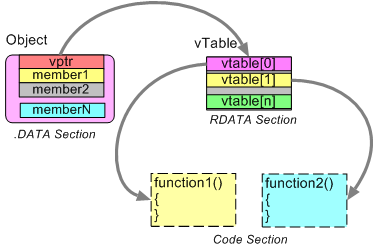
\includegraphics{vtable}
\end{frame}

\begin{frame}{Abstract Classes \& Interfaces}
	\begin{itemize}
		\pause \item An \textbf{Abstract Class} is a class which cannot be initialised but is intended to be used as a base class
		\pause \item It will have at lease one function marked as pure virtual (see example)
		\pause \item If you then inherit from an abstract class, you have to provide an implementation of all pure virtual functions
	\end{itemize}
\end{frame}

\begin{frame}{Abstract Classes \& Interfaces}
	\begin{itemize}
		\pause \item An \textbf{Interface} is very similar to an abstract class, the only difference is that every function in an Interface is marked as pure virtual
		\pause \item If you then inherit from an interface, you have to provide an implementation of all pure virtual functions
	\end{itemize}
\end{frame}

\begin{frame}[fragile]{Abstract Class}
	\begin{lstlisting}[language=C++,basicstyle=\tiny,]
	class BaseEnemy
	{
	public: 
		//Make sure we have a deconstructor defined!
		virtual ~BaseEnemy(){};
		virtual void Attack()=0;
		void Jump()
		{
			//Do jump code
		};
	}
	
	class Orc : public BaseEnemy
	{
		public:
			//we have to implement attack but no need to implement Jump 
			void Attack()
			{
				//do attack
			}
	}
	\end{lstlisting}
\end{frame}

\begin{frame}[fragile]{Interface Example}
	\begin{lstlisting}[language=C++,basicstyle=\tiny,]
	class IJump
	{
	public:
		//We must provide a virtual deconstructor
		virtual ~Jump(){};
		void DoJump()=0;
	}
	
	class IAttack
	{
	public:
		virtual ~Attack(){};
		void DoAttack()=0;
	}
	
	class Orc : public IJump, public IAttack
	{
	//we have to implement Attack and Jump Interface
	public:
		void DoAttack()
		{
			//do attack
		}
		
		void DoJump()
		{
			//do Jump
		}
	}
	\end{lstlisting}
\end{frame}

\begin{frame}{Interface Discussion}
	\begin{itemize}
		\pause \item You can think of an Interface as a contract
		\pause \item The derived class must implement the Interface's function
		\pause \item We can leverage Polymorphism to work with interfaces
		\pause \item This means that I can consume derived classes in a function that takes in pointers to the Interface
	\end{itemize}
\end{frame}

\begin{frame}{Interface Discussion}
	\begin{itemize}
		\pause \item Lastly, Interfaces a great tool for working with others. We as a group could create the interface together
		\pause \item Then another programmer can write Classes which implement the Interface
		\pause \item While another writes code which consumes instances of the Interface 
		\pause \item \url{https://stackoverflow.com/questions/4456424/what-do-programmers-mean-when-they-say-code-against-an-interface-not-an-objec} 
	\end{itemize}
\end{frame}